\chapter{Development/Design and Implementation}\label{cha:dev}

\section{Development Strategy}

The main goal of this study was to create a tool that can automatically classify \gls{DNA} sequences using \gls{ML}/\gls{DL} models, followed by its integration into \textit{ProPythia}. Another important objective was to integrate automated machine learning classifiers into the \textit{OmniumAI} software platforms.

However, it is crucial to understand the steps and the technologies necessary to build such tools.

After selecting the dataset, the first step of an \gls{ML} project is the data processing task since, in most cases, the data is not ready to be fed into a model. The sequences need first to be converted into a numerical representation, and how this step is executed has a substantial influence on the model's ultimate performance. 
As mentioned in section~\ref{sec:workflow}, data processing can be subdivided into feature extraction and feature selection. The first is the process of transforming raw data into suitable modelling features, and the second consists of filtering irrelevant features, keeping the essential ones. If the model is a \gls{DL} model, the user may not need to perform this step since these kind of models can extract the features from the training data on their own.

In this study, descriptors were calculated and used as features for shallow \gls{ML} classification models, which is a manual feature extraction process. For \gls{DL} models, they only need the sequences as input but they still need to be in a numerical format. Encoders were utilized to address this problem since they can create numerical representations of a string of letters.

%%%%%%%%%%%%%%%%%%%%%%%%%%%%%%%%%%%%%%%%%%%%%%%%%%%%%%%%%%%%%%%%%%%%%%%%%%%%%%%%%%%%%%%%%%%%%%%%%%%%%%%%%%%%%%%%%%%%%

\subsection{ProPythia}

As mentioned in section~\ref{sec:context_and_motivation}, \textit{ProPythia} is a platform devoted to the classification of peptides/proteins sequences using \gls{ML} and \gls{DL}, developed within the Biosystems group at CEB/ U. Minho. Included in \textit{ProPythia} are modules to read and modify sequences, calculate various types of protein descriptors, pre-process datasets, execute feature selection and dimensionality reduction, visualize t-SNE and UMAP, perform clustering, train and optimize \gls{ML} and \gls{DL} models, and make predictions using various algorithms. \textit{ProPythia} features an adjustable modular design that makes it a flexible and user-friendly tool for \gls{ML}/\gls{DL} analysis of protein sequences~\cite{Sequeira2020ProPythia:Learning}. A schematic view
of the package can be seen in Figure~\ref{fig:propythia_workflow}.

\begin{figure}[htbp]
    \centering
    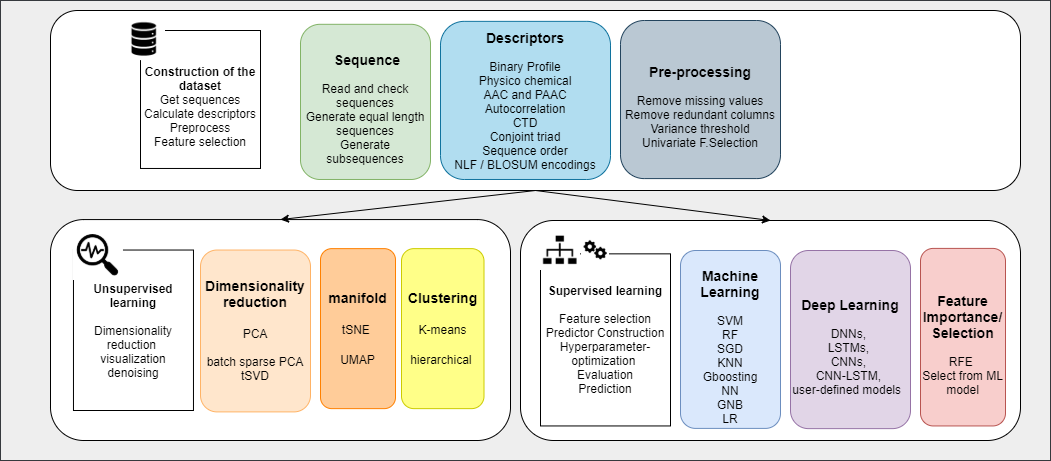
\includegraphics[width=\linewidth]{propythia_workflow}
    \caption{Schematic representation of the modules in ProPythia~\cite{Sequeira2020ProPythia:Learning}.}
    \label{fig:propythia_workflow}
\end{figure}

The first main objective of this study regarding \textit{ProPythia} was to extend its calculation of descriptors for proteins to also include \gls{DNA} descriptors. To accomplish this, a module (similar to the one for proteins) was developed that can be simply imported by other modules to create a \textit{Python} dictionary containing all calculated descriptors. As the remaining \gls{ML} steps are independent of one another, \textit{ProPythia} is now capable of performing the whole \gls{ML} pipeline for \gls{DNA} data. The list of implemented \gls{DNA} descriptors can be found later in section~\ref{cha:descriptors}.

The other key objective was the development of a complete \gls{DL} pipeline for the classification of \gls{DNA} sequences. Although \textit{ProPythia} already includes a module for \gls{DL} classifications, it was not used to complete this step since it was not built in \textit{PyTorch} but rather in \textit{Tensorflow/Keras}.

The implemented \gls{DL} steps were encoding, data processing, model building and training, model evaluation, and finally hyperparameter tuning. Each one of these steps were built as separate independent modules that can be used between themeselves and also between the modules that were already in \textit{ProPythia}. For example, it is possible to use the new \gls{DNA} encodings to train a \textit{ProPythia}'s \gls{DL} model and also use \textit{ProPythia}'s protein encoders to train a \gls{DL} \textit{PyTorch} model. Figure~\ref{fig:meu} provides an overview of the developed workflow.

\begin{figure}[htbp]
    \centering
    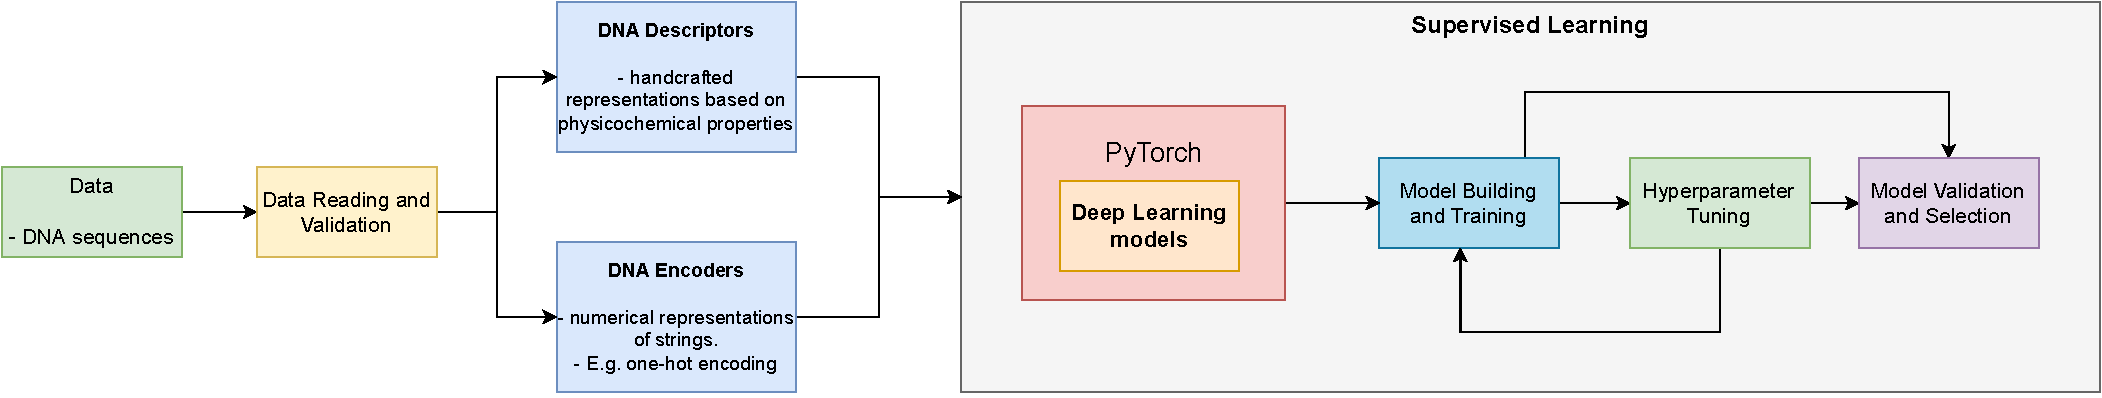
\includegraphics[width=\linewidth]{meu}
    \caption{Implemented workflow in ProPythia for Deep Learning DNA classifications.}
    \label{fig:meu}
\end{figure}

Figure~\ref{fig:integration_propythia} provides a visualization of how the implemented modules of \gls{DL} \gls{DNA} classification is integrated in \textit{Propythia}. The coloured modules were the new ones implemented and the gray ones are from \textit{ProPythia}.

\begin{figure}[htbp]
    \centering
    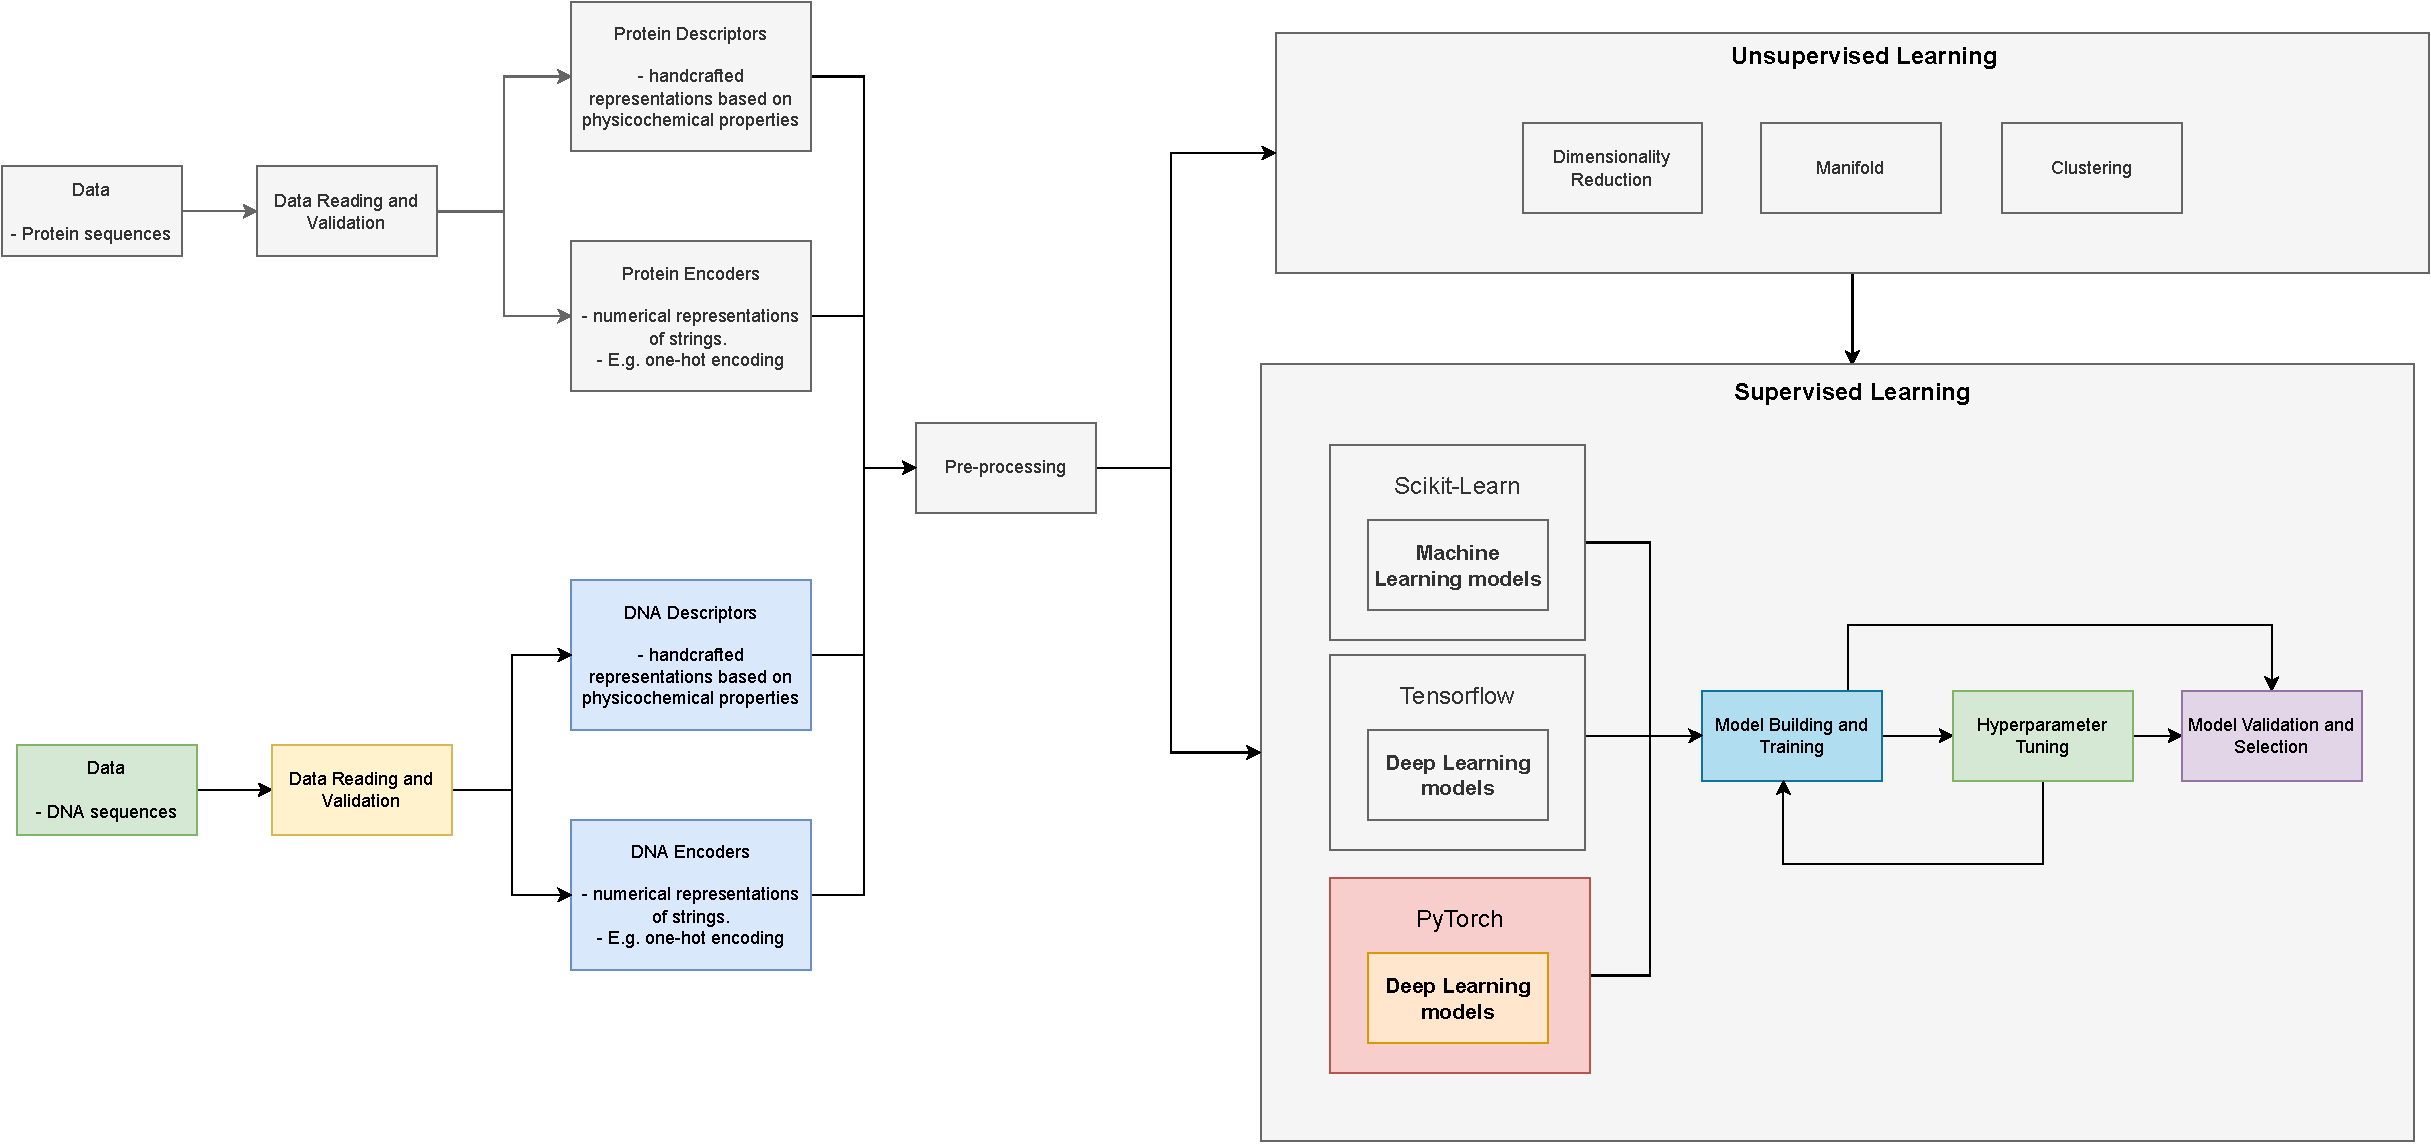
\includegraphics[width=\linewidth]{integration_propythia}
    \caption{Integration of implemented modules in ProPythia.}
    \label{fig:integration_propythia}
\end{figure}

Both implementations of \gls{DNA} descriptors and the \gls{DL} pipeline had a step in common; the data reading process. As a result, a data reading module was developed to read \gls{DNA} sequences from \textit{CSV} or \textit{FASTA} files. The data is then validated, which means that every letter in the sequence has to be either an \gls{A}, \gls{C}, \gls{G}, or \gls{T}.

\subsection{Omnia}

\section{Setting up the Data}\label{sec:setup}

It is important to note that all sequence feature vectors that will be fed into the model need to have the same input shape, regardless of whether the sequences have the same length or not. For example, a sequence with a length of 100 and another sequence with a length of 200, that belong to the same dataset, must be represented by a feature vector of the same size. When using descriptors, this can be achieved by implementing them in a way that they are not dependent on the sequence's length. However, when using encodings, the only option is to truncate or fill all sequences to a length's value. Using the example above, the two sequences could be truncated or filled to have a length of 150, and then calculate the encoding. To fill the sequence to a length's value, a letter that did not belong to the \gls{A}, \gls{C}, \gls{T}, and \gls{G} alphabet was added - the letter N. 

The following chapter provides an overview of the descriptors and the encoders for \gls{DNA} sequences that were developed in this study.

\subsection{Descriptors}\label{cha:descriptors}

Table~\ref{tab:descriptors_classes} provides the list of all the implemented descriptors, as well as their respective group and resulting vector size. The process of obtaining this list of descriptors was based on finding the descriptors that most \gls{DNA} descriptors packages from Table~\ref{tab:descriptors_DNA} implemented, as well as choosing the ones that did not depend on the sequence's length, as the datasets used in the case studies did not have sequences of uniform length.

The $N$ in the table represents the number of physicochemical indices to calculate.


\begin{table}[ht]
	\caption{List of implemented descriptors.}
	\label{tab:descriptors_classes}
    \centering
    \scalebox{0.9}{
    \begin{tabular}{lll}
    	\toprule
    	\textbf{Descriptor groups} & \textbf{Descriptor} & \textbf{Vector Size}\\\midrule
    	
    	\multirow{3}{*}{Psychochemical} & Length & 1\\
    	& GC Content & 1\\
    	& AT Content & 1\\\midrule
    	
    	\multirow{6}{*}{Nucleic Acid Compostion} & Nucleic Acid Compostion (NAC) & 4\\
    	
    	& Dinucleotide Acid Compostion (DNC) & 16\\
    	& Trinucleotide Acid Compostion (TNC) & 64\\
    	& Composition of K-spaced nucleic acid pairs (CKSNAP) & 16\\
    	& K-mer & $4^{k}$\\
    	& Accumulated Nucleotide Frequency (ANF) & $3 * 4$\\\midrule
    	
    	\multirow{6}{*}{Auto Correlation and Cross Covariance} & Dinucleotide-based Auto Covariance (DAC) & $N * lag$\\
    	& Dinucleotide-based Cross Covariance (DCC) & $N * (N-1) * lag$\\
    	& Dinucleotide-based Auto-Cross Covariance (DACC) & $N * N * lag$ \\
    	& Trinucleotide-based Auto Covariance (TAC) & $N * lag$\\
    	& Trinucleotide-based Cross Covariance (TCC) & $N * (N-1) * lag$\\
    	& Trinucleotide-based Auto-Cross Covariance (TACC) & $N * N * lag$\\\midrule
    	
    	\multirow{2}{*}{Pseudo Nucleic Acid Composition} & Pseudo Dinucleotide Compostion (PseDNC) & $16 + \lambda$\\
    	& Pseudo K-tupler Compostion (PseKNC) & $4^{k} + \lambda$\\
    	
        
    	\bottomrule
    \end{tabular}
    }
\end{table}


Both the psychochemical properties and the nucleic acid composition are the most straight-forward approaches to represent the \gls{DNA} sequences. 

\paragraph{Length}

Length descriptor is a simple descriptor that calculates the length of a sequence.

\paragraph{GC Content}

\gls{GC} content feature encoding represents the quantity of guanine and cytosine nucleotides in a sequence. It can be calculated as follows:

\begin{equation}\label{eq:gc_content}
    x = \frac{N_{(C)} + N_{(G)}}{L}
\end{equation}


\noindent where $N_{(C)}$ donates the number of the nucleotide C in the sequence, $N_{(G)}$ the number of the nucleotide G and $L$ the length of the sequence.

\paragraph{AT Content}

\gls{AT} content feature encoding represents the quantity of adenine and thymine nucleotides in a sequence. It can be calculated as follows:


\begin{equation}\label{eq:at_content}
    x = \frac{N_{(A)} + N_{(T)}}{L}
\end{equation}

\noindent where $N_{(A)}$ donates the number of the nucleotide A in the sequence, $N_{(T)}$ the number of the nucleotide T and $L$ the length of the sequence.


\paragraph{Nucleic Acid Composition}

The \gls{NAC} encoding~\cite{Chen2015IRNA-Methyl:Composition,Chen2013IRSpot-PseDNC:Composition} is one of the approaches often used to represent \gls{DNA} sequences; it represents the nucleotide frequencies of the sequence. The frequencies of the 4 natural nucleotides may be determined as follows:

\begin{equation}\label{eq:NAC}
    f(i) = \frac{N_{(i)}}{L}, i \in \left\{A,C,T,G\right\}
\end{equation}

\noindent where $N_{(i)}$ is the number of nucleotide type and $L$ is the length of the \gls{DNA} sequence.

\paragraph{Di-Nucleotide Composition}

\gls{DNC} feature encoding~\cite{Grabherr2011ExploitingPromoters, Panwar2015IdentificationTri-nucleotides} is the composition of continuous dinucleotide pairs inside a \gls{DNA} sequence. \gls{DNC} feature encoding has 16 descriptors, which are specified as follows:

\begin{equation}\label{eq:DNC}
    D(i,j) = \frac{N_{(ij)}}{L-1}, i,j \in \left\{A,C,T,G\right\}
\end{equation}

\noindent where $N_{(ij)}$ is the number of dinucleotide represented by nucleotide types $i$ and $j$, and $L$ is the length of the \gls{DNA} sequence.

\paragraph{Tri-Nucleotide Composition}

\gls{TNC} feature encoding~\cite{Qiu2014IRSpot-TNCPseAAC:Components,Panwar2014PredictionInformation} reflects the \gls{DNA} sequence's composition of continuous trinucleotide pairs. \gls{TNC} feature encoding has 64 descriptors ('AAA', 'AAC', 'AAG', 'AAT',..., 'TTT'), which may be described as follows:

\begin{equation}\label{eq:TNC}
    D(i,j,k) = \frac{N_{(ijk)}}{L-2}, i,j,k \in \left\{A,C,T,G\right\}
\end{equation}

\noindent where $N_{(ijk)}$ is the number of trinucleotides represented by nucleotide types $i$, $j$ and $k$, and $L$ is the length of the \gls{DNA} sequence.


\paragraph{Composition of K-spaced nucleic acid pairs}

\gls{CKSNAP} feature encoding~\cite{Zhang2013PredictionPairs,Liu2017BioSeq-Analysis:Approaches} denotes the composition of nucleotide pairs in a segment that are K-steps apart. Specifically, we estimated the frequency of a nucleotide pair at positions $i$ and $i + K + 1$, where $i$ = 1,..., ($l$ - $K$ - 1) and $l$ is the length of the sequence. For instance, given the sequence $ACGTACGT$ and $K$ = 2, the nucleotide AT will appear twice, with A and T occurring at positions 1 and 4, as well as positions 5 and 8.
Regardless of the number of $K$, there are a maximum of 16 potential nucleotide pairings. This coding method represents the close interactions between nucleic acids inside a \gls{DNA} sequence segment.

\paragraph{K-mer}

The K-mer encoding~\cite{Manavalan20194mCpred-EL:Genome,Huang2018BERMP:Approach} determines the occurrence frequencies of K adjacent nucleotides in a \gls{DNA} sequence, which was widely employed in enhancer discovery and regulatory sequence prediction. The K-mer (e.g. K = 4) descriptor is described as follows:

\begin{equation}\label{eq:K-mer}
    K(i) = \frac{N_{(i)}}{L}, i \in \left\{AAAA, AAAC, AAAG,...,TTTT\right\}
\end{equation}

\noindent where $N_{i}$ is the number of K-tuple type and $L$ is the length of the \gls{DNA} sequence.

The K-mer descriptor implemented additionally contains the \gls{RCKmer}. The \gls{RCKmer} encoding~\cite{Chen2019ILearn:Data} is a variation of the K-mer descriptor that computes the occurrence frequencies of reverse complement k adjacent nucleotides in a \gls{DNA} sequence. For example, a \gls{DNA} sequence has 16 types of 2-mers. Among them, 'TT' is the opposite of 'AA'. By deleting the reverse complimentary K-mers, there are only 10 varieties of 2-mers in the \gls{RCKmer} method (i.e. 'AA', 'AC', 'AG', 'AT', 'CA', 'CC', 'CG', 'GA', 'GC', and 'TA').

\paragraph{Accumulated Nucleotide Frequency}

\gls{ANF} feature encoding technique~\cite{Feng2019IDNA6mA-PseKNC:PseKNC} represents the nucleotide density and distribution of each nucleotide inside a \gls{DNA} segment. The following formula illustrates how to determine the \gls{ANF} of a \gls{DNA} segment of length $K$.

\begin{equation}\label{eq:ANF}
    d_{l} = \frac{1}{l}\sum_{j=1}^{l}f(n_{j}), f(n_{j}) = \begin{cases}1 & n_{j} = q\\0 & other\end{cases}, l = 1,...,K
\end{equation}

\noindent where $n_{j}$ is the nucleotide at the $j^{th}$ position and $q \in (A,C,T,G)$. When $l$ = 3, the nucleotide at the $l^{th}$ position in the sequence of 'TGCTACGC' is C, and the density of this position is calculated as $d_{3} = \frac{1}{3}\sum_{j=1}^{3}f(n_{j}) = \frac{1}{3} [f(C) + f(A) + f(C)] = \frac{1}{3} [1+0+1] = 0.667$. All $K$ locations' densities may be estimated identically. When computing the \gls{ANF} at each place, however, there would be $K$ values, which is not a vector of constant length. To circumvent this, the \gls{ANF} was only computed for three places located at 25, 50, and 75\% of the sequence's length.

\paragraph{Dinucleotide-based Auto-covariance}

The first autocorrelation descriptor is called \gls{DAC}. As one of the multivariate modeling methods, autocorrelation can turn \gls{DNA} sequences of varying lengths into vectors of constant length by assessing the correlation between any two physicochemical variables. Autocorrelation generates two types of variables: autocorrelation (AC) between the same property and cross-covariance (CC) between properties with different values.

It has been proved that \gls{DNA} physicochemical properties play important roles in gene expression regulation~\cite{Brukner1995Sequence-dependentTrinucleotides.,Fukue2005ARelevance}. 

There are 38 dinucleotide physicochemical properties and 12 trinucleotide physicochemical properties listed in Table \ref{tab:38_di} and Table~\ref{tab:12_tri}, respectively, that may be utilized to construct distinct modes of dinucleotide and trinucleotide autocorrelation features. The present analysis was confined to dinucleotide and trinucleotide autocorrelation descriptors since little physicochemical property data are available for K-tuple nucleotides with $K = 4$ and higher. When the necessary physicochemical property data are available, however, the formulae described here may be simply modified to include the scenario when $K \geq 4$~\cite{Chen2014PseKNC:Composition}.


\begin{footnotesize}
    \begin{longtable}{ccc}
        \caption{List of 38 physicochemical properties of dinucleotides in DNA.~\cite{Chen2014PseKNC:Composition}}
        \label{tab:38_di}
        \endfirsthead
        \endhead
        \toprule
        \textbf{Number} & \textbf{Description}\\\midrule
        
        1 & Base stacking	\\\midrule
        2 & Protein-induced deformability	\\\midrule
        3 & B-DNA twist	\\\midrule
        4 & Dinucleotide GC content	\\\midrule
        5 & A-philicity	\\\midrule
        6 & Propeller twist	\\\midrule
        7 & Duplex stability (free energy)	\\\midrule
        8 & Duplex stability (disrupt energy)	\\\midrule
        9 & DNA denaturation	\\\midrule
        10 & Bending stiffness	\\\midrule
        11 & Protein-DNA twist	\\\midrule
        12 & Stabilizing energy of Z-DNA	\\\midrule
        13 & Aida\_BA\_transition	\\\midrule
        14 & Breslauer\_dG	\\\midrule
        15 & Breslauer\_dH	\\\midrule
        16 & Breslauer\_dS	\\\midrule
        17 & Electron interaction	\\\midrule
        18 & Hartman\_trans\_free\_energy	\\\midrule
        19 & Helix-coil\_transition	\\\midrule
        20 & Ivanov\_BA\_transition	\\\midrule
        21 & Lisser\_BZ\_transition	\\\midrule
        22 & Polar\_interaction	\\\midrule
        23 & SantaLucia\_dG	\\\midrule
        24 & SantaLucia\_dH	\\\midrule
        25 & SantaLucia\_dS	\\\midrule
        26 & Sarai\_flexibility	\\\midrule
        27 & Stability	\\\midrule
        28 & Stacking\_energy	\\\midrule
        29 & Sugimoto\_dG	\\\midrule
        30 & Sugimoto\_dH	\\\midrule
        31 & Sugimoto\_dS	\\\midrule
        32 & Watson-Crick\_interaction	\\\midrule
        33 & Twist	\\\midrule
        34 & Tilt	\\\midrule
        35 & Roll	\\\midrule
        36 & Shift	\\\midrule
        37 & Slide	\\\midrule
        38 & Rise	\\
        
        \bottomrule
        
    \end{longtable}
\end{footnotesize}
    
\begin{footnotesize}
    \begin{longtable}{ccc}
        \caption{List of 12 physicochemical properties of trinucleotides in DNA.~\cite{Chen2014PseKNC:Composition}}
        \label{tab:12_tri}
        \endfirsthead
        \endhead
        \toprule
        \textbf{Number} & \textbf{Description}\\\midrule
        
        1	& Bendability (DNase)	\\\midrule
        2	& Bendability (consensus)	\\\midrule
        3	& Trinucleotide GC content	\\\midrule
        4	& Nucleosome positioning	\\\midrule
        5	& Consensus-roll \\\midrule
        6	& Consensus-rigid \\\midrule
        7	& DNase I	\\\midrule
        8	& DNase I-rigid	\\\midrule
        9	& MW-daltons	\\\midrule
        10	& MW-kg \\\midrule
        11	& Nucleosome	\\\midrule
        12	& Nucleosome-rigid	\\
        
        \bottomrule
        
    \end{longtable}
\end{footnotesize}

Consider a \gls{DNA} sequence $D$ containing $L$ nucleic acid residues, i.e.

\begin{equation}\label{eq:d-seq}
    D = R_{1}\;R_{2}\;R_{3}\;...\;R_{L}
\end{equation}

\noindent where $R_{i}$ is the nucleic acid residue at the sequence position $i \in [1,2,...,L]$ and $L$ is the length of the \gls{DNA} sequence. The \gls{DAC} evaluates the correlation of the same physicochemical index between two dinucleotides separated by a distance of lag in the sequence. This correlation can be determined as follows:

\begin{equation}\label{eq:DAC}
    DAC(u,lag) = \frac{\sum_{i=1}^{L-lag-1}(P_{u}(R_{i}\;R_{i+1}) - \overline{P_{u}})(P_{u}(R_{i+lag}\;R_{i+lag+1}) - \overline{P_{u}})}{L-lag-1}
\end{equation}

\noindent where $u$ is a physicochemical index, $L$ is the length of the \gls{DNA} sequence, $P_{u}(R_{i}R_{i+1})$ is the numerical value of the physicochemical index $u$ for the dinucleotide $R_{i}R_{i+1}$ at the $i^{th}$ position, and $\overline{P_{u}}$ is the average value for physicochemical index $u$ in the sequence~\cite{Zhu2016RDNAse:CHINA}. The latter is calculated as follows:

\begin{equation}\label{eq:DAC-PU}
    \overline{P_{u}} = \frac{\sum_{j=1}^{L-1}P_{u}(R_{j}R_{j+1})}{L-1}
\end{equation}

The length of \gls{DAC} feature vector is $N*LAG$, where $N$ is the number of physicochemical indices and $LAG$ is the maximum of $lag, lag \in [1,2,...,LAG]$~\cite{Zhu2016RDNAse:CHINA}.

\paragraph{Dinucleotide-based Cross Covariance}
Given a \gls{DNA} sequence D (Eq~\ref{eq:d-seq}), the \gls{DCC} method examines the correlation between two distinct physicochemical indices between two dinucleotides separated by lag nucleic acids in the sequence. This correlation may be determined using:

\begin{equation}\label{eq:DCC}
    DCC(u_{1},u_{2},lag) = \frac{\sum_{i=1}^{L-lag-1}(P_{u_{1}}(R_{i}\;R_{i+1}) - \overline{P_{u_{1}}})(P_{u_{2}}(R_{i+lag}\;R_{i+lag+1}) - \overline{P_{u_{2}}})}{L-lag-1}
\end{equation}

\noindent where $u_{1}$, $u_{2}$ are two different physicochemical indices, $L$ is the length of the \gls{DNA} sequence, \\
$P_{u_{1}}(R_{i}R_{i+1}) (P_{u_{2}}(R_{i}R_{i+1}))$ is the physicochemical index value $u_{1}(u_{2})$ for the dinucleotide $R_{i}R_{i+1}$ $i^{th}$ position, and $\overline{P_{u_{1}}}\;(\overline{P_{u_{2}}})$ is the average value for physicochemical index value $u_{1}$, $u_{2}$ along in the sequence:

\begin{equation}\label{eq:DAC-PU2}
    \overline{P_{u}} = \frac{\sum_{j=1}^{L-1}P_{u}(R_{j}R_{j+1})}{L-1}
\end{equation}

The length of \gls{DCC} feature vector is $N*(N-1)*LAG$, where $N$ is the number of physicochemical indices and $LAG$ is the maximum of $lag, lag \in [1,2,...,LAG]$.

\paragraph{Dinucleotide-based Auto-Cross Covariance}
Combining \gls{DAC} and \gls{DCC} results in \gls{DACC}, meaning the length of the \gls{DACC} vector is $N*N*LAG$, where $N$ is the number of physicochemical indices and $LAG$ is the maximum of $lag, lag \in [1,2,...,LAG]$.


\paragraph{Trinucleotide-based Auto Covariance}
Given a \gls{DNA} sequence D (Eq.~\ref{eq:d-seq}), the \gls{TCC} method examines the correlation of the same physicochemical index between two trinucleotides separated by \textit{lag} nucleic acids in the sequence. This correlation may be determined using:

\begin{equation}\label{eq:tac}
    TAC(lag,u) = 
\frac
{
\sum_{i=1}^{L-lag-2}(P_{u}(R_{i}R_{i+1}R_{i+2}) - \overline{P_{u}})(P_{u}(R_{i+lag}R_{i+lag+1}R_{i+lag+2}) - \overline{P_{u}})
}
{
L-lag-2
}
\end{equation}

\noindent where $u$ is a physicochemical index, $L$ is the length of the \gls{DNA} sequence, $P_{u}(R_{i}R_{i+1}R_{i+2})$ is the numerical value of the physicochemical index $u$ for the trinucleotide $R_{i}R_{i+1}R_{i+2}$ at $i^{th}$ position, $\overline{P_{u}}$ is the average value for physicochemical index $u$ along the whole sequence:

\begin{equation}\label{eq:tac-2}
    \overline{P_{u}} = \frac{\sum_{j=1}^{L-2}P_{u}(R_{j}R_{j+1}R_{j+2})}{L-2}
\end{equation}

The length of \gls{TAC} feature vector is $N*LAG$, where $N$ is the number of physicochemical indices and $LAG$ is the maximum of $lag, lag \in [1,2,...,LAG]$.

\paragraph{Trinucleotide-based Cross Covariance}

Given a \gls{DNA} sequence D (Eq.~\ref{eq:d-seq}), the \gls{TCC} method examines the correlation of two different physicochemical indices between two trinucleotides separated by \textit{lag} nucleic acids in the sequence. This correlation may be determined using:

\begin{equation}\label{eq:TCC}
    TCC(u_{1},u_{2},lag) = \frac{\sum_{i=1}^{L-lag-2}(P_{u_{1}}(R_{i}\;R_{i+1}\;R_{i+2}) - \overline{P_{u_{1}}})(P_{u_{2}}(R_{i+lag}\;R_{i+lag+1}\;R_{i+lag+2}) - \overline{P_{u_{2}}})}{L-lag-2}
\end{equation}

\noindent where $u_{1}$, $u_{2}$ are two different physicochemical indices, $L$ is the length of the \gls{DNA} sequence, \\ $P_{u_{1}}(R_{i}R_{i+1}R_{i+2}) (P_{u_{2}}(R_{i}R_{i+1}R_{i+2}))$ is the numerical value of the physicochemical index $u_{1}(u_{2})$ for the trinucleotide $R_{i}R_{i+1}R_{i+2}$ at $i^{th}$ position, $\overline{P_{u_{1}}}\;(\overline{P_{u_{2}}})$ is the average value for physicochemical index value $u_{1}$, $u_{2}$ in the sequence:

\begin{equation}\label{eq:TCC-PU2}
    \overline{P_{u}} = \frac{\sum_{j=1}^{L-2}P_{u}(R_{j}R_{j+1}R_{j+2})}{L-2}
\end{equation}

The length of \gls{TCC} feature vector is $N*(N-1)*LAG$, where $N$ is the number of physicochemical indices and $LAG$ is the maximum of $lag, lag \in [1,2,...,LAG]$.


\paragraph{Trinucleotide-based Auto-Cross Covariance}
Combining \gls{TAC} and \gls{TCC} results in \gls{TACC}, meaning the length of the \gls{TACC} feature vector is $N*N*LAG$, where $N$ is the number of physicochemical indices and $LAG$ is the maximum of $lag, lag \in [1,2,...,LAG]$.

\paragraph{Pseudo Dinucleotide Composition}

% https://academic.oup.com/nar/article/41/6/e68/2902382
% https://www.ncbi.nlm.nih.gov/pmc/articles/PMC8138820/

All of the mentioned techniques relied only on the composition of nucleic acids, ignoring the influence of sequence order. \gls{PseDNC} is an approach incorporating the contiguous local sequence-order information and the global sequence-order information into the feature vector of the \gls{DNA} sequence. 

Given a \gls{DNA} sequence D (Eq.~\ref{eq:d-seq}), if the feature vector of D is formulated by its \gls{NAC}, we have:

%%%%%%%%%%%%%%%%%%%%%%%%%%%%%%%%%%%%%%%%%%%%%%%%%%%%%%%%%%%%%%%%%%%%%%%%%%%%%%%%%%

\begin{equation}\label{eq:PseDNC-0}
    D = [f(A)\;f(C)\;f(G)\;f(T)]^{T}
\end{equation}

\noindent where $f(A)$, $f(C)$, $f(G)$ and $f(T)$ are the normalized occurrence frequencies of the nucleotides in the \gls{DNA} sequence and the $T$ is the transpose operator symbol. As shown by Eq. \ref{eq:PseDNC-0}, all the sequence-order information is lost when a \gls{DNA} sequence is represented by \gls{NAC}. If the \gls{DNC} is used to represent the \gls{DNA} sequence, rather than the four components provided in~\ref{eq:PseDNC-0}, the associated feature vector will have $4 * 4 = 16$ components, as shown in the following equation.

\begin{equation}\label{eq:PseDNC-1-1}
    D = [f(AA)\;f(AC)\;...\;f(TT)]^{T} = [f_{1}\;f_{2} \;...\;f_{16}]^{T}
\end{equation}

\noindent where each element is the normalized occurrence frequency of the dinucleotide in the \gls{DNA} sequence. Eq.~\ref{eq:PseDNC-1-1} contains the most contiguous local sequence-order information, but the formulation does not take into account any of the global sequence-order data.

The global sequence-order information may be included into the feature vector for the \gls{DNA} sequence using the procedure that follows.

\begin{equation}\label{eq:PseDNC-thetas}
    \begin{cases}
    \theta_{1} = \frac{1}{L-2} \sum_{i=1}^{L-2}\Theta(R_{i}R_{i+1}, R_{i+1}R_{i+2})
    \\ 
    \theta_{2} = \frac{1}{L-3} \sum_{i=1}^{L-3}\Theta(R_{i}R_{i+1}, R_{i+2}R_{i+3})
    \\ 
    \theta_{3} = \frac{1}{L-4} \sum_{i=1}^{L-4}\Theta(R_{i}R_{i+1}, R_{i+3}R_{i+4}) & (\lambda < L)
    \\
    ...
    \\ 
    \theta_{\lambda} = \frac{1}{L-1-\lambda} \sum_{i=1}^{L-1-\lambda}\Theta(R_{i}R_{i+1}, R_{i+\lambda}R_{i+\lambda+1})
    \end{cases}
\end{equation}

\noindent where $\theta_{1}$ is the first-tier correlation factor that represents the sequence-order correlation between all the most contiguous dinucleotides in a sequence (Figure~\ref{fig:psednc_correlation}A); $\theta_{2}$, the second-tier correlation factor between all the second most contiguous dinucleotides (Figure~\ref{fig:psednc_correlation}B); $\theta_{3}$, the third-tier correlation factor between all the third most contiguous dinucleotides (Figure~\ref{fig:psednc_correlation}C) and so forth~\cite{Chen2013IRSpot-PseDNC:Composition}.

\begin{figure}[htbp]
    \centering
    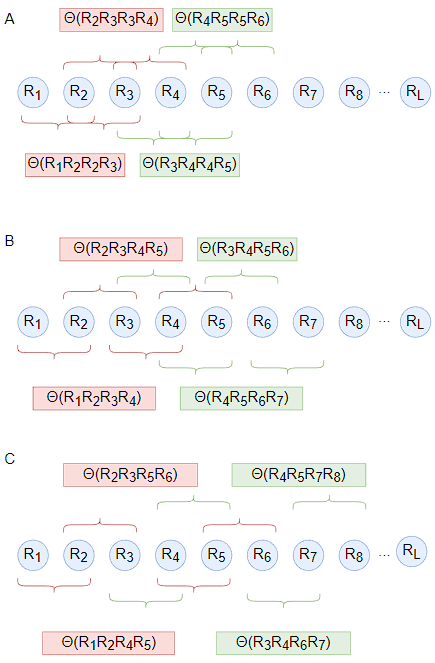
\includegraphics[width=0.75\linewidth]{correlation_di}
    \caption{Correlations of dinucleotides along a DNA sequence. Adapted from~\cite{Chen2013IRSpot-PseDNC:Composition}}
    \label{fig:psednc_correlation}
\end{figure}


In Eq.~\ref{eq:PseDNC-thetas}, the parameter $\lambda$ is an integer that represents the correlation along a \gls{DNA} sequence that has the greatest counted tier, and the correlation function is provided by:

\begin{equation}\label{eq:PseDNC-5}
    \Theta(R_{i}R_{i+1}, R_{j}R_{j+1}) = \frac{1}{\mu}\sum_{u=1}^{\mu}[P_{u} (R_{i}R_{i+1}) - P_{u}(R_{j}R_{j+1})]^{2}
\end{equation}

\noindent where $\mu$ is the number of local \gls{DNA} structural features taken into account in the current investigation, which is equal to six. $P_{u} (R_{i}R_{i+1})$ represents the numerical value of the \textit{u-th} $(u = 1,2,...,\mu)$ \gls{DNA} local property for the dinucleotide $R_{i}R_{i+1}$ at position $i$. And $P_{u}(R_{j}R_{j+1})$ is the corresponding value for the dinucleotide $R_{j}R_{j+1}$ at position $j$.

Numerous lines of research have shown that certain local \gls{DNA} structural properties, such as angular parameters (twist, tilt, and roll) and translational parameters (shift, slide, and rise), play significant roles in biological processes, including protein-\gls{DNA} interactions, chromosome formation, and higher-order organization of the genetic material~\cite{Goni2008DNAlive:Scale,Goni2007DeterminingCalculations}. Listed in Table \ref{tab:original_numerical} are the original numerical values for twist $P_{1}(R_{i}R_{i+1})$⁠, tilt $P_{2}(R_{i}R_{i+1})$⁠, roll $P_{3}(R_{i}R_{i+1})$⁠, shift $P_{4}(R_{i}R_{i+1})$⁠, slide $P_{5}(R_{i}R_{i+1})$⁠, and rise $P_{6}(R_{i}R_{i+1})$⁠, respectively, where $R_{i}R_{i+1}$ represents the 16 possible dinucleotides. Only these six \gls{DNA} local physical structural properties were used to calculate \gls{PseDNC}, explaining why $\mu = 6$ in Eq.~\ref{eq:PseDNC-5}.

\begin{table}[ht]

    \caption{Original numerical values for the six DNA dinucleotide physical structures~\cite{Chen2013IRSpot-PseDNC:Composition}}
    \label{tab:original_numerical}
    
    \centering
    \begin{tabular}{ccccccc}

        \toprule
        \textbf{Dinucleotide} & $P_{1}(R_{i}R_{i+1})$ & $P_{2}(R_{i}R_{i+1})$ & $P_{3}(R_{i}R_{i+1})$ & $P_{4}(R_{i}R_{i+1})$ & $P_{5}(R_{i}R_{i+1})$ & $P_{6}(R_{i}R_{i+1})$\\\midrule

        AA & 0.026  & 0.038 & 0.020 & 1.69 & 2.26 & 7.65 \\\midrule
        AC & 0.036  & 0.038 & 0.023 & 1.32 & 3.03 & 8.93 \\\midrule
        AG & 0.031  & 0.037 & 0.019 & 1.46 & 2.03 & 7.08 \\\midrule
        AT & 0.033  & 0.036 & 0.022 & 1.03 & 3.83 & 9.07 \\\midrule
        CA & 0.016  & 0.025 & 0.017 & 1.07 & 1.78 & 6.38 \\\midrule
        CC & 0.026  & 0.042 & 0.019 & 1.43 & 1.65 & 8.04 \\\midrule
        CG & 0.014  & 0.026 & 0.016 & 1.08 & 2.00 & 6.23 \\\midrule
        CT & 0.031  & 0.037 & 0.019 & 1.46 & 2.03 & 7.08 \\\midrule
        GA & 0.025  & 0.038 & 0.020 & 1.32 & 1.93 & 8.56 \\\midrule
        GC & 0.025  & 0.036 & 0.026 & 1.20 & 2.61 & 9.53 \\\midrule
        GG & 0.026  & 0.042 & 0.019 & 1.43 & 1.65 & 8.04 \\\midrule
        GT & 0.036  & 0.038 & 0.023 & 1.32 & 3.03 & 8.93 \\\midrule
        TA & 0.017  & 0.018 & 0.016 & 0.72 & 1.20 & 6.23 \\\midrule
        TC & 0.025  & 0.038 & 0.020 & 1.32 & 1.93 & 8.56 \\\midrule
        TG & 0.016  & 0.025 & 0.017 & 1.07 & 1.78 & 6.38 \\\midrule
        TT & 0.026  & 0.038 & 0.020 & 1.69 & 2.26 & 7.65 \\

        \bottomrule
    \end{tabular}
\end{table}

Prior to inserting into Eq.~\ref{eq:PseDNC-5}, the values listed in Table~\ref{tab:original_numerical} were adjusted through a standard conversion~\cite{Chou2005UsingClasses}, as shown by the equation below:

\begin{equation}\label{eq:PseDNC-6}
    P_{u}(R_{i}R_{i+1}) = \frac{P_{u}(R_{i}R_{i+1}) - <P_{u}>}{SD(P_{u})}
\end{equation}

\noindent where the symbol $<>$ is averaging the amount present for each of the 16 dinucleotides, (Eq.~\ref{eq:PseDNC-1-1}), and $SD$ is the corresponding standard deviation. Table~\ref{tab:normalized_values} provides the normalized values of $P_{u}(R_{i}R_{i+1})\;(u = 1,2,...,6)$ which were derived using the standard conversion calculation (Eq.~\ref{eq:PseDNC-6}) from the Table~\ref{tab:original_numerical} original values.

\begin{table}[ht]

    \caption{The normalized values for the six DNA dinucleotide physical structures
    ~\cite{Chen2013IRSpot-PseDNC:Composition}}
    \label{tab:normalized_values}
    
    \centering
    \begin{tabular}{ccccccc}

        \toprule
        \textbf{Dinucleotide} & $P_{1}(R_{i}R_{i+1})$ & $P_{2}(R_{i}R_{i+1})$ & $P_{3}(R_{i}R_{i+1})$ & $P_{4}(R_{i}R_{i+1})$ & $P_{5}(R_{i}R_{i+1})$ & $P_{6}(R_{i}R_{i+1})$\\\midrule
        
        AA & 0.06  &	0.5 	& 0.27 	& 1.59 	& 0.11 	& -0.11 \\\midrule
        AC & 1.50  &	0.50 	& 0.80 	& 0.13 	& 1.29 	& 1.04 \\\midrule
        AG & 0.78  &	0.36 	& 0.09 	& 0.68 	& -0.24 & -0.62 \\\midrule
        AT & 1.07  &	0.22 	& 0.62 	& -1.02 & 2.51 	& 1.17 \\\midrule
        CA & -1.38 & 	-1.36 	& -0.27 & -0.86 & -0.62 & -1.25 \\\midrule
        CC & 0.06  &	1.08 	& 0.09 	& 0.56 	& -0.82 & 0.24 \\\midrule
        CG & -1.66 & 	-1.22 	& -0.44 & -0.82 & -0.29 & -1.39 \\\midrule
        CT & 0.78  &	0.36 	& 0.09 	& 0.68 	& -0.24 & -0.62 \\\midrule
        GA & -0.08 & 	0.5 	& 0.27 	& 0.13 	& -0.39 & 0.71 \\\midrule
        GC & -0.08 & 	0.22 	& 1.33 	& -0.35 & 0.65 	& 1.59 \\\midrule
        GG & 0.06  &	1.08 	& 0.09 	& 0.56 	& -0.82 & 0.24 \\\midrule
        GT & 1.50  &	0.50 	& 0.80 	& 0.13 	& 1.29 	& 1.04 \\\midrule
        TA & -1.23 & 	-2.37 	& -0.44 & -2.24 & -1.51 & -1.39 \\\midrule
        TC & -0.08 & 	0.5 	& 0.27 	& 0.13 	& -0.39 & 0.71 \\\midrule
        TG & -1.38 & 	-1.36 	& -0.27 & -0.86 & -0.62 & -1.25 \\\midrule
        TT & 0.06  &	0.5 	& 0.27 	& 1.59 	& 0.11 	& -0.11 \\

        \bottomrule
    \end{tabular}
\end{table}

It is conceivable to draw the conclusion that a collection of sequence-correlation factors $\theta_{1},...,\theta_{\lambda}$ defined by Eq.~\ref{eq:PseDNC-thetas} and \ref{eq:PseDNC-5}, may represent the sequence-order effect of a \gls{DNA} sequence. The process for augmenting the \gls{DNC} of Eq.~\ref{eq:PseDNC-1-1} to the \gls{PseDNC} is similar to that described in~\cite{Chou2001PredictionComposition} for changing the amino acid composition to the \gls{PseACC}.

\begin{equation}\label{eq:PseDNC-8}
    D = [d_{1}\;d_{2}\;...\;d_{16}\;d_{16+1}\;...\;d_{16+\lambda}]^{T}
\end{equation}

\noindent where

\begin{equation}\label{eq:PseDNC-9}
    d_{k} = \begin{cases}\frac{f_{k}}{\sum_{i=1}^{16} f_{i} + w\sum_{j=1}^{\lambda}\theta_{j}} & 1 \le k \le 16\\\frac{w\theta_{k-16}}{\sum_{i=1}^{16} f_{i} + w\sum_{j=1}^{\lambda}\theta_{j}} & 17 \le k \le 16 + \lambda\end{cases}
\end{equation}

\noindent where $f_{k}$ is normalized occurrence frequency of the $k$-th dinucleotide in the sequence, $\theta_{j}$ is given by Eq.~\ref{eq:PseDNC-thetas}, $\lambda$ represents the number of tiers of the correlations in the sequence and $w$ is the weight factor. As a result, instead of a 16-dimensional vector (Eq.~\ref{eq:PseDNC-1-1}), the \gls{DNA} sequence is formed by a $(16 + \lambda) - D$ vector as stated in Eq.~\ref{eq:PseDNC-8}. The \gls{DNA} sequences with very different lengths may be turned into a collection of feature vectors with the same dimension thanks to the extra $\lambda$ correlation factors, in addition to allowing for the inclusion of significant global sequence-order effects. This last requirement is crucial since many classification engines demand a collection of vectors with a certain number of components as input.

%%%%%%%%%%%%%%%%%%%%%%%%%%%%%%%%%%%%%%%%%%%%%%%%%%%%%%%%%%%%%%%%%%%%%%%%%%%%%%%%%%%%%%%%%%%%%%%%%%%%%%%%%%%%%%%%%%%%%%%%%%%%%%%%%%%%%%%%%%%%%%%%%%%%%%%%%%%%%%%%%%%%%%%%%%%%%%%%%%%%%%%%%%%%%%%%%%%%%%%%%%%%%%%%%%%%%%%%%%%%%%%%%%%%%%%%%%%%%%%%%%%%%%%%%%%%%%%%%%%%%%%%%%%%%%

\paragraph{Pseudo K-tupler Composition}

% https://github.com/liufule12/repDNA/blob/master/repDNA/doc/repDNA_manual.pdf

\gls{PseKNC} is the enhanced version of \gls{PseDNC} by adding k-tuple nucleotide composition.

Given a \gls{DNA} sequence D (Eq.~\ref{eq:d-seq}), the feature vector of D is defined:

\begin{equation}\label{eq:PseKNC-feature-vector}
    D = [d_{1}\;d_{2}\;...\;d_{4^{k}}\;d_{4^{k+1}}\;...\;d_{4^{k+ \lambda}}]^{T}
\end{equation}

\noindent where

\begin{equation}\label{eq:PseKNC-du}
    d_{u} = 
    \begin{cases}
        \frac{f_{u}}{\sum_{i=1}^{4^{k}} f_{i} + w\sum_{j=1}^{\lambda}\theta_{j}} & 1 \le u \le 4^{k}
    \\
        \frac{w\theta_{u-4^{k}}}{\sum_{i=1}^{4^{k}} f_{i} + w\sum_{j=1}^{\lambda}\theta_{j}} & 4^{k} \le u \le 4^{k} + \lambda
    
    \end{cases}
\end{equation}

\noindent where $\lambda$ is the number of tiers of the correlations in a sequence; $f_{u}$ is the normalized occurrence frequency of the $u$-th dinucleotide in the sequence; $w$ is a weight factor; $\theta_{j}$ is given by:

\begin{equation}\label{eq:PseKNC-thetas}
\theta_{j} = \frac{1}{L-j-1} \sum_{i=1}^{L-j-1}\Theta(R_{i}R_{i+1}, R_{i+j}R_{i+j+1}), \;j\in{1,2,...,\lambda;\lambda < L}
\end{equation}

\noindent which is the $j$-tier structural correlation factor between all the $j^{th}$ most
contiguous dinucleotides. The correlation function $\Theta(R_{i}R_{i+1}, R_{i+j}R_{i+j+1})$ is defined by:

\begin{equation}\label{eq:PseKNC-correlation}
    \Theta(R_{i}R_{i+1}, R_{i+j}R_{i+j+1}) = \frac{1}{\mu}\sum_{v=1}^{\mu}[P_{v} (R_{i}R_{i+1}) - P_{v}(R_{i+j}R_{i+j+1})]^{2}
\end{equation}

\noindent where $\mu$ is the number of physicochemical indices reflecting the local \gls{DNA} structural properties (Table~\ref{tab:normalized_values}); $P_{v} (R_{i}R_{i+1})$ is the value of the $v^{th}$ physicochemical indice for the dinucleotide $R_{i}R_{i+1}$ at $i^{th}$ position and $P_{v} (R_{i+j}R_{i+j+1})$ is the corresponding value for the dinucleotide $R_{i+j}R_{i+j+1}$ at $(i+j)^{th}$ position.

\subsection{Encoders}

\gls{DNA} sequences consist of continuous sequential letters from a 4-letter alphabet, and, as mentioned in Section~\ref{sec:dna-dl}, it is first required to transform the string sequence into a numerical value in order to create an input matrix for the model. However, as mentioned in Section~\ref{sec:setup}, an additional letter was included in the alphabet in order to fill sequences to a determined length - the letter N.

The encoders implemented were one-hot encoding, chemical encoding and k-mer one-hot encoding.

\paragraph{One-Hot Encoding}

One-hot encoding is extensively used in deep learning models and is well suited for most models. In addition, the performance of one-hot encoding is very stable across various data sets. However, an appropriate model is necessary to get acceptable performance. This approach preserves the positional information of each nucleotide in sequences but disregards high-order relationships between nucleotides and previous biological information~\cite{Zhang2019ModelingNetwork}.

As a result, \gls{A} is encoded to (1, 0, 0, 0), \gls{C} to (0, 1, 0, 0), \gls{G} to (0, 0, 1, 0), \gls{T} to (0, 0, 0, 1), and N to (0, 0, 0, 0). The final vector's dimension will be $L * 4$ where $L$ is the length of the sequence.

\paragraph{Chemical Encoding}

The four nucleic acids each have unique chemical characteristics~\cite{GolamBari2013DNASequence}. \gls{A} and \gls{G} are purines with two ring structures, whereas \gls{C} and \gls{T} are pyrimidines with one ring structure. \gls{C} and \gls{G} create strong hydrogen bonds while building secondary structures, whereas \gls{A} and \gls{T} form weak hydrogen bonds. In terms of their chemical functionality, \gls{A} and \gls{C} belong to the amino group, while \gls{G} and \gls{T} belong to the keto group. Accordingly, the four nucleic acids may be categorized into three separate categories (Table~\ref{tab:chemical_encoding}).

\begin{table}[ht]
	\caption{Cluster of nucleotides based on chemical properties~\cite{GolamBari2013DNASequence}}
	\label{tab:chemical_encoding}
    \centering
    \begin{tabular}{lll}
    	\toprule
    	\textbf{Chemical property} & \textbf{Class} & \textbf{Nucleotides} \\\midrule
    	
    	\multirow{2}{*}{Ring structure} & Purine & A,G \\
    	& Pyrimidine & C,T\\\midrule
    	
    	\multirow{2}{*}{Hydrogen bond} & Weak & A,T\\
    	& Strong & C,G\\\midrule
    	
    	\multirow{2}{*}{Functional group} & Amino & A,C\\
    	& Keto & G,T\\
        
    	\bottomrule
    \end{tabular}
\end{table}

Three coordinates $(x, y, z)$ were utilized to represent the chemical characteristics of the four nucleotides, and the values 0 and 1 were given to the coordinates in order to incorporate these attributes. If $x$, $y$, and $z$ coordinates respectively represent the ring structure, the hydrogen bond, and the chemical functionality, then each nucleotide may be encoded as ($x_{i}$, $y_{i}$, $z_{i}$), where $x_{i}$ represents the ring structure, $y_{i}$ represents the hydrogen bond, and $z_{i}$ represents the chemical functionality.

As a result, \gls{A} is encoded to (1, 1, 1), \gls{C} to (0, 0, 1), \gls{G} to (1, 0, 0), \gls{T} to (0, 1, 0) and N to (0, 0, 0). The final vector's dimension will be $L * 3$ where $L$ is the length of the sequence.


\paragraph{K-mer One-Hot Encoding}

As mentioned before, using one-hot encoding on \gls{DNA} sequences solely preserves the positional information of each nucleotide. Recent investigations, however, have shown that including high-order dependencies among nucleotides may enhance the efficacy of \gls{DNA} models~\cite{Zhang2019ModelingNetwork}. To capture the dependencies, all instances are turned into image-like matrices of high-order relationships using the k-mer encoding method.

For example, in 1-mer one-hot encoding, each nucleotide is mapped into a vector of size 5 ($A = [1, 0, 0, 0, 0]^{T}$, $C = [0, 1, 0, 0, 0]^{T}$, $G = [0, 0, 1, 0 ,0]^{T}$, $T = [0, 0, 0, 1, 0]^{T}$, and $N = [0, 0, 0, 0, 1]^{T}$). The 2-mer one hot encoding is based on the dependencies between two nearby nucleotides, and each dinucleotide is mapped to a 25-dimensional vector ($AA = [1, 0, 0, ..., 0]^{T}$, ..., $NN = [0, 0, 0, ..., 1]^{T})$. The 3-mer one hot encoding is based on the dependencies between three nearby nucleotides, and each trinucleotide is mapped to a 125-dimensional vector ($AAA = [1, 0, 0, 0, ..., 0, 0, 0, 0, 0]^{T}$, ... , $NNN = [0, 0, 0, 0, ..., 0, 0, 0, 0, 0, 1]^{T}$).

As a result, the final vector's dimension will be $(L - k + 1) * 5^{k}$ where $L$ is the length of the sequence.

\section{Classifiers Implementation}

Following the selection of the dataset, the \gls{DNA} sequence records were randomly rearranged and assigned to the training and test/validation sets. A suitable data preprocessing strategy was selected in order to turn the \gls{DNA} sequences, into a numerical representation. This format was necessary to comply with the input requirements of the classification model, which takes only numerical data.

At this stage, there will be either a collection of pre-calculated features, the descriptors, or labeled and encoded training data. The data will be used to train the classification model regardless of the previous choice.

\subsection{Models}

The following sections will provide an insight for each one of the implemented classification models.

\paragraph{MLP}

Usa descritores. Dizer que há 2 versões 

\paragraph{CNN}

Usa encodings. Dizer que há 2 versões 

\paragraph{LSTM / BiLSTM}

Usa encodings

\paragraph{GRU / BiGRU}

Usa encodings

\paragraph{CNN-LSTM / CNN-BiLSTM}

Usa encodings

\paragraph{CNN-GRU / CNN-BiGRU}

Usa encodings

\subsection{Hyperparameter Tuning}

Additionally, hyperparameter optimization was considered and applied successfully. As mentioned in~\ref{sec:workflow}, the challenge of hyperparameter optimization is selecting the appropriate hyperparameters for a learning algorithm. It may distinguish an ordinary model from a very accurate one. Choosing a different learning rate or modifying the size of a network layer may have a substantial effect on the performance of the model. Ray Tune~\cite{Liaw2018Tune:Training} is the standard tuning tool for hyperparameters and it was used to complete this task. However, before finding the best combination, it is required to define the configuration of the Ray Tune's search space. The implemented one can be found in Table~\ref{tab:search_space}.

\begin{table}[ht]
	\caption{Ray Tune's search space.}
	\label{tab:search_space}
    \centering
    \begin{tabular}{lll}
    	\toprule
    	\textbf{Hyperparameter (x)} & \textbf{Search Space} & \textbf{Models} \\\midrule
    	
    	Hidden Size & $x \in 32, 64, 128, 256$ & All\\\midrule
        Batch Size & $x \in 8, 16, 32, 64$ & All\\\midrule
        Learning Rate & $x \in 0.0001, 0.001, 0.01$ & All\\\midrule
        Dropout & $x \in 0.2, 0.3, 0.4, 0.5$ & All\\\midrule
        Number of Layers & $x \in 1, 2, 3$ & All\\
        
    	\bottomrule
    \end{tabular}
\end{table}

Ray Tune will now randomly choose a combination of parameters from these search areas for each trial. It will then train many models in parallel and determine which one has the highest performance. Additionally, the Ray Tune's scheduler \textit{ASHAScheduler} was used, which terminates poorly performing trials early. This is accomplished by choosing a desired metric (loss in this study) and measuring it at the end of each epoch. If the measure keeps worsening, reaching a specified patience value, the trial will end immediately. 

\subsection{Other Parameters}

The process of early stopping is a very useful technique since it prevents wasting time and resources on unnecessary computations. Therefore, this strategy was also implemented in the case when hyperparameter tuning is not being performed, using now the \textit{ReduceLROnPlateau} scheduler from \textit{PyTorch}. This scheduler is also able to reduce the learning rate when the given metric has stopped improving, since models often benefit from a 2-10x reduction in the learning rate when learning has stagnated.

\section{Technologies used}

This section will go through the main technologies employed in this project that were very crucial in achieving the final result.

\subsection{The Software}

\textit{Python} is a high-level interpreted general-purpose programming language that supports vast and extensive external libraries that are constantly evolving. \textit{PyCharm Code Editor} was used to combine Python code development while also improving usability and user experience. Additionally, the \textit{Anaconda} software application was employed to facilitate package management and distribution.

\subsection{The Hardware}

\subsection{The Libraries}

PyTorch and Tensorflow are the most popular and powerful \gls{ML} frameworks, and one had to be chosen to be used in this research for the implementation of the models. 

%%%%%%%%%%%%%%%%%%%%%%%%%%%%%%%%%%%%%%%%%%%%%%%%%%%%%%%%%%%%%%%%%%%%%%%%%%%%%%%%%%%%%%%%
%% VER SE VALE A PENA DIZER O PORQUE DE TER SIDO ESCOLHIDO PYTORCH EM VEZ DE KERAS / TENSFORFLOW
%%%%%%%%%%%%%%%%%%%%%%%%%%%%%%%%%%%%%%%%%%%%%%%%%%%%%%%%%%%%%%%%%%%%%%%%%%%%%%%%%%%%%%%%%%%%%%%%%%%%%%%%%%%%%%%%%%%%%%%%

\textit{PyTorch} is a free and open-source \gls{ML}/\gls{DL} library that was used in this research to create the all the models. 

\textit{Numpy} is a key Python library for scientific computing that supports massive, multidimensional arrays, complex matrix arithmetic, and much more. This package was highly helpful for data pre-processing as well as matrix arithmetic calculation in the classication model.

Last but not least, \textit{Matplotlib} is a \textit{Python} package used to plot 2D graphs and other high-quality figures. The latter were based on data obtained from the classication model.